\newpage
\section{Lecture 4: Fitting Models and Optimization Algorithms}

\subsection{Fitting Models}
We want to fit a model family to data by optimizing a loss function.
Dataset:
\[
\mathcal{D}=\{(\mathbf{x}_i,y_i)\}_{i=1}^{I}.
\]
Model:
\[
\hat{y}_i=f(\mathbf{x}_i;\boldsymbol{\phi}).
\]
Loss:
\[
L(\boldsymbol{\phi})=\sum_{i=1}^{I}\ell_i(\boldsymbol{\phi})
=\sum_{i=1}^{I}\ell\!\left(y_i,f(\mathbf{x}_i;\boldsymbol{\phi})\right).
\]
Goal:
\[
\hat{\boldsymbol{\phi}}=\arg\min_{\boldsymbol{\phi}}L(\boldsymbol{\phi}).
\]

\subsection{Probabilistic View and Maximum Likelihood}
Step 1: model conditional probability
\[
p(y\mid \mathbf{x},\boldsymbol{\theta}).
\]
Step 2: parameterize with a network output
\[
\boldsymbol{\theta}_i = f(\mathbf{x}_i;\boldsymbol{\psi}).
\]
Step 3: maximize log-likelihood:
\[
\hat{\boldsymbol{\psi}}
=
\arg\max_{\boldsymbol{\psi}}
\sum_{i=1}^{I}\log p(y_i\mid \boldsymbol{\theta}_i).
\]
Equivalent minimization:
\[
\hat{\boldsymbol{\psi}}
=
\arg\min_{\boldsymbol{\psi}}
\left[-\sum_{i=1}^{I}\log p(y_i\mid \boldsymbol{\theta}_i)\right].
\]

Gaussian example:
\[
y_i\mid \mathbf{x}_i \sim \mathcal{N}\!\left(\mu_i,\sigma^2\right),
\qquad
\mu_i=f(\mathbf{x}_i;\boldsymbol{\phi}).
\]
Then minimizing negative log-likelihood gives least squares.

\subsection{Gradient Descent (GD)}
Update rule:
\[
\boldsymbol{\phi}_{t+1}
=
\boldsymbol{\phi}_t
-\alpha\nabla_{\boldsymbol{\phi}}L(\boldsymbol{\phi}_t),
\]
where $\alpha$ is the step size (learning rate).

\textbf{Three-step view:}
\begin{itemize}
    \item Step 0: initialize $\boldsymbol{\phi}_0$
    \item Step 1: compute gradient $\nabla_{\boldsymbol{\phi}}L(\boldsymbol{\phi}_t)$
    \item Step 2: update $\boldsymbol{\phi}\leftarrow \boldsymbol{\phi}-\alpha\nabla_{\boldsymbol{\phi}}L$
\end{itemize}

\subsection{Square Loss Example (Linear Regression)}
Model:
\[
f(x;\boldsymbol{\phi})=\phi_0+\phi_1x.
\]
Loss:
\[
L(\boldsymbol{\phi})
=
\sum_{i=1}^{I}\left(\phi_0+\phi_1x_i-y_i\right)^2.
\]
Full derivatives:
\[
\frac{\partial L}{\partial \phi_0}
=
2\sum_{i=1}^{I}\left(\phi_0+\phi_1x_i-y_i\right),
\]
\[
\frac{\partial L}{\partial \phi_1}
=
2\sum_{i=1}^{I}\left(\phi_0+\phi_1x_i-y_i\right)x_i.
\]
Vector update:
\[
\begin{bmatrix}\phi_0\\\phi_1\end{bmatrix}_{t+1}
=
\begin{bmatrix}\phi_0\\\phi_1\end{bmatrix}_{t}
-\alpha
\begin{bmatrix}
\partial L/\partial \phi_0\\
\partial L/\partial \phi_1
\end{bmatrix}_{t}.
\]

\subsection{Convex vs Non-Convex Loss}
Convex losses have one global minimum (for linear least squares in standard form).
Deep models are generally non-convex and can have many local minima/saddle points.

\begin{figure}[h!]
\centering
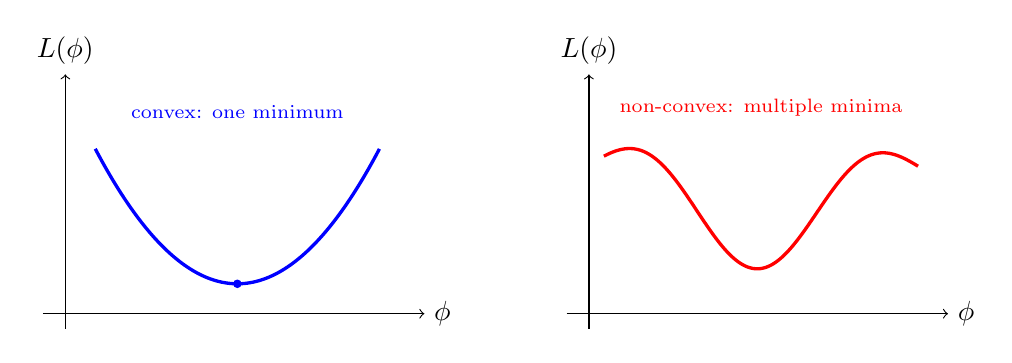
\begin{tikzpicture}[scale=0.95]
    % Left: convex
    \begin{scope}[xshift=0cm]
        \draw[->] (-0.3,0) -- (4.8,0) node[right] {$\phi$};
        \draw[->] (0,-0.2) -- (0,3.2) node[above] {$L(\phi)$};
        \draw[very thick,blue,domain=0.4:4.2,samples=100]
            plot (\x,{0.5*(\x-2.3)^2+0.4});
        \filldraw[blue] (2.3,0.4) circle (1.4pt);
        \node[blue] at (2.3,2.7) {\scriptsize convex: one minimum};
    \end{scope}
    % Right: non-convex
    \begin{scope}[xshift=7cm]
        \draw[->] (-0.3,0) -- (4.8,0) node[right] {$\phi$};
        \draw[->] (0,-0.2) -- (0,3.2) node[above] {$L(\phi)$};
        \draw[very thick,red,domain=0.2:4.4,samples=200]
            plot (\x,{1.2 + 0.6*sin(deg(2.1*\x)) + 0.15*(\x-2.3)^2});
        \node[red] at (2.3,2.75) {\scriptsize non-convex: multiple minima};
    \end{scope}
\end{tikzpicture}
\caption{Optimization landscape: convex (left) vs non-convex (right).}
\end{figure}

\subsection{Stochastic Gradient Descent (SGD)}
Instead of full dataset each step, use a mini-batch $B_t\subset\{1,\dots,I\}$:
\[
\mathbf{g}_t
=
\frac{1}{|B_t|}
\sum_{i\in B_t}\nabla_{\boldsymbol{\phi}}\ell_i(\boldsymbol{\phi}_t),
\qquad
\boldsymbol{\phi}_{t+1}=\boldsymbol{\phi}_t-\alpha\mathbf{g}_t.
\]

\textbf{Epoch:} one full pass over all training examples.
If dataset size is $I$ and batch size is $b$, then one epoch has about
\[
\left\lceil\frac{I}{b}\right\rceil
\]
parameter updates.

\begin{figure}[h!]
\centering
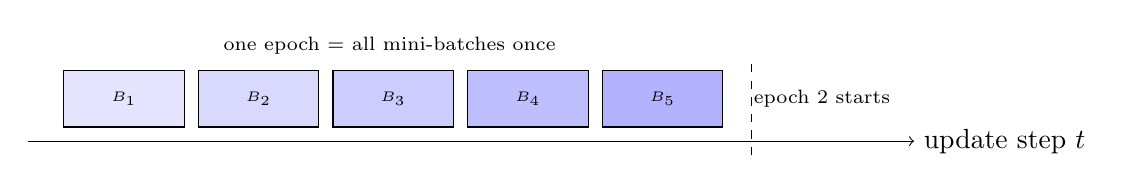
\begin{tikzpicture}[scale=0.9]
    % Time axis
    \draw[->] (0,0) -- (12.5,0) node[right] {update step $t$};

    % Batch blocks across one epoch
    \draw[fill=blue!10] (0.5,0.2) rectangle (2.2,1.0);
    \draw[fill=blue!15] (2.4,0.2) rectangle (4.1,1.0);
    \draw[fill=blue!20] (4.3,0.2) rectangle (6.0,1.0);
    \draw[fill=blue!25] (6.2,0.2) rectangle (7.9,1.0);
    \draw[fill=blue!30] (8.1,0.2) rectangle (9.8,1.0);
    \node at (5.1,1.35) {\scriptsize one epoch = all mini-batches once};

    \node at (1.35,0.6) {\tiny $B_1$};
    \node at (3.25,0.6) {\tiny $B_2$};
    \node at (5.15,0.6) {\tiny $B_3$};
    \node at (7.05,0.6) {\tiny $B_4$};
    \node at (8.95,0.6) {\tiny $B_5$};

    % Next epoch marker
    \draw[dashed] (10.2,-0.2) -- (10.2,1.2);
    \node at (11.2,0.6) {\scriptsize epoch 2 starts};
\end{tikzpicture}
\caption{Mini-batch SGD timeline and the meaning of an epoch.}
\end{figure}

\subsection{Hyperparameters}
Hyperparameters are chosen outside optimization, for example:
\begin{itemize}
    \item learning rate $\alpha$
    \item batch size $b$
    \item number of epochs
    \item optimizer parameters ($\beta$, $\beta_1$, $\beta_2$, $\epsilon$)
\end{itemize}

\subsection{SGD with Momentum}
Momentum tracks an exponentially weighted average of gradients:
\[
\mathbf{m}_{t+1}=\beta\mathbf{m}_t+(1-\beta)\mathbf{g}_t,
\qquad
\mathbf{g}_t=\frac{1}{|B_t|}\sum_{i\in B_t}\nabla\ell_i(\boldsymbol{\phi}_t),
\]
\[
\boldsymbol{\phi}_{t+1}=\boldsymbol{\phi}_t-\alpha\mathbf{m}_{t+1}.
\]
Interpretation: updates become smoother and continue in consistent descent
directions, reducing zig-zag behavior. Momentum includes history and can be viewed
as an infinite weighted sum of past gradients.

\paragraph{Example up to \texorpdfstring{$m_3$}{m3}.}
Assume scalar gradients and $\beta=0.9$, $m_0=0$, with
$g_1=2.0$, $g_2=1.0$, $g_3=1.5$:
\[
m_1=0.9\cdot 0+0.1\cdot 2.0=0.2,
\]
\[
m_2=0.9\cdot 0.2+0.1\cdot 1.0=0.28,
\]
\[
m_3=0.9\cdot 0.28+0.1\cdot 1.5=0.402.
\]
So the update at step 3 uses $\alpha m_3$, not just $\alpha g_3$.

\subsection{Graph: Without vs With Momentum}
\begin{figure}[h!]
\centering
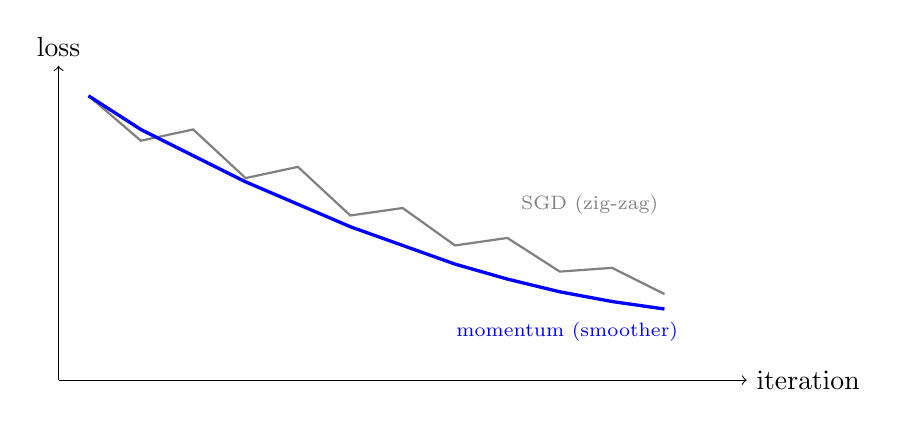
\begin{tikzpicture}[scale=0.95]
    % Axes
    \draw[->] (0,0) -- (9.2,0) node[right] {iteration};
    \draw[->] (0,0) -- (0,4.2) node[above] {loss};

    % Plain SGD (noisy)
    \draw[thick,gray]
        (0.4,3.8)--(1.1,3.2)--(1.8,3.35)--(2.5,2.7)--(3.2,2.85)--(3.9,2.2)--(4.6,2.3)--(5.3,1.8)--(6.0,1.9)--(6.7,1.45)--(7.4,1.5)--(8.1,1.15);
    \node[gray] at (7.1,2.35) {\scriptsize SGD (zig-zag)};

    % Momentum (smoother)
    \draw[very thick,blue]
        (0.4,3.8)--(1.1,3.35)--(1.8,3.0)--(2.5,2.65)--(3.2,2.35)--(3.9,2.05)--(4.6,1.8)--(5.3,1.55)--(6.0,1.35)--(6.7,1.18)--(7.4,1.05)--(8.1,0.95);
    \node[blue] at (6.8,0.65) {\scriptsize momentum (smoother)};
\end{tikzpicture}
\caption{Momentum smooths SGD updates by using past gradient information.}
\end{figure}

\subsection{Nesterov Accelerated Gradient (NAG)}
Nesterov evaluates gradient at a look-ahead point:
\[
\tilde{\boldsymbol{\phi}}_t=\boldsymbol{\phi}_t-\alpha\beta\mathbf{m}_t,
\]
\[
\mathbf{m}_{t+1}=\beta\mathbf{m}_t+(1-\beta)\nabla L(\tilde{\boldsymbol{\phi}}_t),
\]
\[
\boldsymbol{\phi}_{t+1}=\boldsymbol{\phi}_t-\alpha\mathbf{m}_{t+1}.
\]
Compared with classical momentum, NAG reacts earlier to changes in curvature.

\subsection{Adam (Adaptive Moment Estimation)}
Adam combines momentum (first moment) and adaptive scaling (second moment):
\[
\mathbf{m}_{t+1}=\beta_1\mathbf{m}_t+(1-\beta_1)\mathbf{g}_t,
\]
\[
\mathbf{v}_{t+1}=\beta_2\mathbf{v}_t+(1-\beta_2)\mathbf{g}_t\odot\mathbf{g}_t.
\]
Bias-corrected moments:
\[
\hat{\mathbf{m}}_{t+1}=\frac{\mathbf{m}_{t+1}}{1-\beta_1^{t+1}},
\qquad
\hat{\mathbf{v}}_{t+1}=\frac{\mathbf{v}_{t+1}}{1-\beta_2^{t+1}}.
\]
Update:
\[
\boldsymbol{\phi}_{t+1}
=
\boldsymbol{\phi}_t
-\alpha\frac{\hat{\mathbf{m}}_{t+1}}{\sqrt{\hat{\mathbf{v}}_{t+1}}+\epsilon}.
\]
Here $\epsilon$ stabilizes division, and $\beta_1,\beta_2$ control averaging.
This gives per-parameter step-size control using squared gradients.

\subsection{Practical Notes}
\begin{itemize}
    \item GD is stable but expensive on large datasets.
    \item SGD is fast per step but noisy.
    \item Momentum and Nesterov improve directionality and speed.
    \item Adam is often robust with minimal tuning, especially in deep networks.
    \item Depth is fixed by architecture; optimizer hyperparameters control training behavior.
\end{itemize}
